\subsubsection{求解与结果分析：硅厚度与碳化硅修正判断}

\begingroup
\renewcommand{\baselinestretch}{1.10}\selectfont

双角光谱先确定硅厚度，再区分谱形改善和测厚影响。

逐次往返厚度对照给出硅全量厚度$2.17\ \mu\mathrm{m}$，对应每角$5392$个原始点。
% src:求解/问题3/结果/解读核验_回炉3_仲裁后.json:防泄漏.全量每角点数
% src:求解/问题3/结果/回炉轮3候选/仲裁闭环/20260910_131501_81623_建模公式/厚度结果.json:核心指标.硅全量完整往返厚度_um

两折厚度为$1.73$和$16.04\ \mu\mathrm{m}$，相差$14.31\ \mu\mathrm{m}$，区段切分改变了硅厚度分支。
% src:求解/问题3/结果/解读核验_回炉3_仲裁后.json:防泄漏.每角抽样点数
% src:求解/问题3/结果/回炉轮3候选/仲裁闭环/20260910_131501_81623_建模公式/厚度结果.json:核心指标.硅折1完整往返条件厚度_um;核心指标.硅折2完整往返条件厚度_um

同段比较沿用$1200$--$3800\ \mathrm{cm}^{-1}$主拟合窗口。为隔开背景变化，两场同阶响应；训练估参、校准定区间、测试评分。
% 依据:交接/建模笔记_问题3.md:5.算法、验证和区间
% src:交接/结果声明_问题3.json:口径说明.硅全量完整往返厚度_um

完整往返场的四附件汇总误差$1.0231$高于两束的$0.9812$，两种朴素对照的误差并列于表\ref{tab:08}。这里先按各角训练残差的四分位距标准化，再对全部角块等权平均，分数为无量纲。
% src:求解/问题3/结果/回炉轮3候选/仲裁闭环/20260910_131501_81623_建模公式/厚度结果.json:分材料验证.硅.逐折汇总.0.平均标准化均方根误差.两束;分材料验证.硅.逐折汇总.0.平均标准化均方根误差.完整往返;分材料验证.硅.逐折汇总.0.平均标准化均方根误差.训练均值;分材料验证.硅.逐折汇总.0.平均标准化均方根误差.二次趋势;分材料验证.硅.逐折汇总.1.平均标准化均方根误差.两束;分材料验证.硅.逐折汇总.1.平均标准化均方根误差.完整往返;分材料验证.硅.逐折汇总.1.平均标准化均方根误差.训练均值;分材料验证.硅.逐折汇总.1.平均标准化均方根误差.二次趋势;分材料验证.碳化硅.逐折汇总.0.平均标准化均方根误差.两束;分材料验证.碳化硅.逐折汇总.0.平均标准化均方根误差.完整往返;分材料验证.碳化硅.逐折汇总.0.平均标准化均方根误差.训练均值;分材料验证.碳化硅.逐折汇总.0.平均标准化均方根误差.二次趋势;分材料验证.碳化硅.逐折汇总.1.平均标准化均方根误差.两束;分材料验证.碳化硅.逐折汇总.1.平均标准化均方根误差.完整往返;分材料验证.碳化硅.逐折汇总.1.平均标准化均方根误差.训练均值;分材料验证.碳化硅.逐折汇总.1.平均标准化均方根误差.二次趋势

同一搜索预算下，完整场仍未降低总体误差。两模型保留原粗候选对照，并在相同条件内整合近优分支、从原始起点精修，采用相同的响应设置。分别估参后的分数差反映两种模型的预测表现；固定参数的场差与重估后的厚度差另行区分，以免把参数补偿解释为纯粹的高阶作用。采用值与计算文件的对应关系见附录\ref{sec:appendix-q3}，两场公式与候选选择分别列出。
% 采用入口：求解/问题3/求解_问题3.py；候选整合版本v3r3；基础场引擎版本v3。

\begingroup
\renewcommand{\baselinestretch}{1.05}
\footnotesize
\setlength{\LTpre}{2pt}
\setlength{\LTpost}{2pt}
\renewcommand{\arraystretch}{1.02}
\begin{longtable}{>{\centering\arraybackslash}p{0.24\textwidth} >{\centering\arraybackslash}p{0.32\textwidth} >{\centering\arraybackslash}p{0.36\textwidth}}
\caption{求解设置与两材料厚度前后对照}\label{tab:08}\\
\hline
核对项目 & 数值或设置 & 对象与含义\\
\hline
初始共同搜索 & $61$个粗候选、$3$个起点 & 原候选保留作共同对照\\
配对精修 & 每起点$150/300$次两级评估 & 两模型均重估五个物理量\\
硅全量厚度 & $2.32\rightarrow2.17\ \mu\mathrm{m}$ & 同段两束$\rightarrow$完整往返场\\
硅折间厚度 & $1.73$、$16.04\ \mu\mathrm{m}$ & 每角$480$点，两次连续切分\\
硅模型厚度差 & $-0.15\ \mu\mathrm{m}$ & 全量完整往返减两束\\
硅条件包络 & $1.72$--$18.16\ \mu\mathrm{m}$ & 非概率的已算情景范围\\
碳化硅同段厚度 & $2.79\rightarrow2.83\ \mu\mathrm{m}$ & 同步重估光学参数\\
碳化硅采用厚度 & $10.80\rightarrow10.80\ \mu\mathrm{m}$ & 实际处理前$\rightarrow$处理后\\
碳化硅采用范围 & $0.64$--$18.11\ \mu\mathrm{m}$（保持） & 前后沿用厚度重估范围\\
留段标准化误差 & $0.9812\rightarrow1.0231$ & 四附件两束$\rightarrow$完整往返场\\
朴素对照误差 & $2.1929$、$1.4434$ & 训练均值、二次趋势\\
高阶可观测性 & 复杂模型适配，仪器资料缺失 & 改善来源未分离\\
稳定测厚影响 & 光学参数与模型影响混合 & 碳化硅不替换基准\\
\hline
\end{longtable}
% src:求解/问题3/结果/回炉轮3候选/仲裁闭环/20260910_131501_81623_建模公式/厚度结果.json:核心指标.硅全量完整往返厚度_um;核心指标.硅折1完整往返条件厚度_um;核心指标.硅折2完整往返条件厚度_um;核心指标.硅已计算条件包络下限_um;核心指标.硅已计算条件包络上限_um;核心指标.碳化硅正式基准厚度_um;核心指标.碳化硅正式条件范围下限_um;核心指标.碳化硅正式条件范围上限_um
% src:求解/问题3/结果/回炉轮3候选/仲裁闭环/20260910_131501_81623_建模公式/厚度结果.json:案例.0.最优.厚度_um;案例.1.最优.厚度_um;案例.6.最优.厚度_um;案例.7.最优.厚度_um
% src:求解/问题3/结果/公平对照.json:案例.0.搜索状态.共同粗候选数;案例.0.搜索状态.共同初值
% src:求解/问题3/结果/回炉轮3候选/仲裁闭环/20260910_131501_81623_建模公式/厚度结果.json:案例.1.分级端点.0.评估上限;案例.1.分级端点.3.评估上限
\endgroup
% 依据:交接/建模笔记_问题3.md:5.算法、验证和区间
% src:求解/问题3/结果/回炉轮3候选/仲裁闭环/20260910_131501_81623_建模公式/厚度结果.json:案例.0.最优.厚度_um;案例.6.最优.厚度_um;案例.7.最优.厚度_um
% src:求解/问题3/结果/解读核验_回炉3_仲裁后.json:防泄漏.每角抽样点数
% src:求解/问题3/结果/回炉轮3候选/仲裁闭环/20260910_131501_81623_建模公式/厚度结果.json:核心指标.硅全量完整往返厚度_um;核心指标.硅折1完整往返条件厚度_um;核心指标.硅折2完整往返条件厚度_um;核心指标.碳化硅正式基准厚度_um;核心指标.碳化硅正式条件范围下限_um;核心指标.碳化硅正式条件范围上限_um
% src:求解/问题3/结果/回炉轮3候选/仲裁闭环/20260910_131501_81623_建模公式/厚度结果.json:分材料验证.硅.逐折汇总.0.平均标准化均方根误差.两束;分材料验证.硅.逐折汇总.0.平均标准化均方根误差.完整往返;分材料验证.硅.逐折汇总.0.平均标准化均方根误差.训练均值;分材料验证.硅.逐折汇总.0.平均标准化均方根误差.二次趋势;分材料验证.硅.逐折汇总.1.平均标准化均方根误差.两束;分材料验证.硅.逐折汇总.1.平均标准化均方根误差.完整往返;分材料验证.硅.逐折汇总.1.平均标准化均方根误差.训练均值;分材料验证.硅.逐折汇总.1.平均标准化均方根误差.二次趋势;分材料验证.碳化硅.逐折汇总.0.平均标准化均方根误差.两束;分材料验证.碳化硅.逐折汇总.0.平均标准化均方根误差.完整往返;分材料验证.碳化硅.逐折汇总.0.平均标准化均方根误差.训练均值;分材料验证.碳化硅.逐折汇总.0.平均标准化均方根误差.二次趋势;分材料验证.碳化硅.逐折汇总.1.平均标准化均方根误差.两束;分材料验证.碳化硅.逐折汇总.1.平均标准化均方根误差.完整往返;分材料验证.碳化硅.逐折汇总.1.平均标准化均方根误差.训练均值;分材料验证.碳化硅.逐折汇总.1.平均标准化均方根误差.二次趋势
% src:求解/问题3/结果/条件判定.json:必要条件;碳化硅条件分支

硅首折同一测试块中，附件三的预测误差由$0.4281$降至$0.3000$个百分点，附件四由$1.0923$降至$0.8759$个百分点。这一局部改善需与全部测试块合看；图\ref{fig:16}承担同段预测与残差的对照。
% src:求解/问题3/结果/回炉轮3候选/仲裁闭环/20260910_131501_81623_建模公式/厚度结果.json:逐块评分.0.均方根误差_反射率比例;逐块评分.4.均方根误差_反射率比例;逐块评分.2.均方根误差_反射率比例;逐块评分.6.均方根误差_反射率比例
% src:求解/问题3/结果/回炉轮3候选/仲裁闭环/20260910_131501_81623_建模公式/厚度结果.json:预测区间.4.经验覆盖率;预测区间.4.平均区间宽度_比例;预测区间.5.经验覆盖率;预测区间.5.平均区间宽度_比例;预测区间.6.经验覆盖率;预测区间.6.平均区间宽度_比例;预测区间.7.经验覆盖率;预测区间.7.平均区间宽度_比例;预测区间.20.经验覆盖率;预测区间.20.平均区间宽度_比例;预测区间.21.经验覆盖率;预测区间.21.平均区间宽度_比例;预测区间.22.经验覆盖率;预测区间.22.平均区间宽度_比例;预测区间.23.经验覆盖率;预测区间.23.平均区间宽度_比例;预测区间.36.经验覆盖率;预测区间.36.平均区间宽度_比例;预测区间.37.经验覆盖率;预测区间.37.平均区间宽度_比例;预测区间.38.经验覆盖率;预测区间.38.平均区间宽度_比例;预测区间.39.经验覆盖率;预测区间.39.平均区间宽度_比例;预测区间.52.经验覆盖率;预测区间.52.平均区间宽度_比例;预测区间.53.经验覆盖率;预测区间.53.平均区间宽度_比例;预测区间.54.经验覆盖率;预测区间.54.平均区间宽度_比例;预测区间.55.经验覆盖率;预测区间.55.平均区间宽度_比例;预测区间.4.名义覆盖率
% src:求解/问题3/结果/回炉轮3候选/仲裁闭环/20260910_131501_81623_建模公式/厚度结果.json:逐块评分.4.测试点数;逐块评分.5.测试点数;逐块评分.6.测试点数;逐块评分.7.测试点数;逐块评分.20.测试点数;逐块评分.21.测试点数;逐块评分.22.测试点数;逐块评分.23.测试点数;逐块评分.36.测试点数;逐块评分.37.测试点数;逐块评分.38.测试点数;逐块评分.39.测试点数;逐块评分.52.测试点数;逐块评分.53.测试点数;逐块评分.54.测试点数;逐块评分.55.测试点数

\begingroup
\setlength{\intextsep}{2pt}
\captionsetup{skip=3pt}
\begin{figure}[!htb]
  \centering
  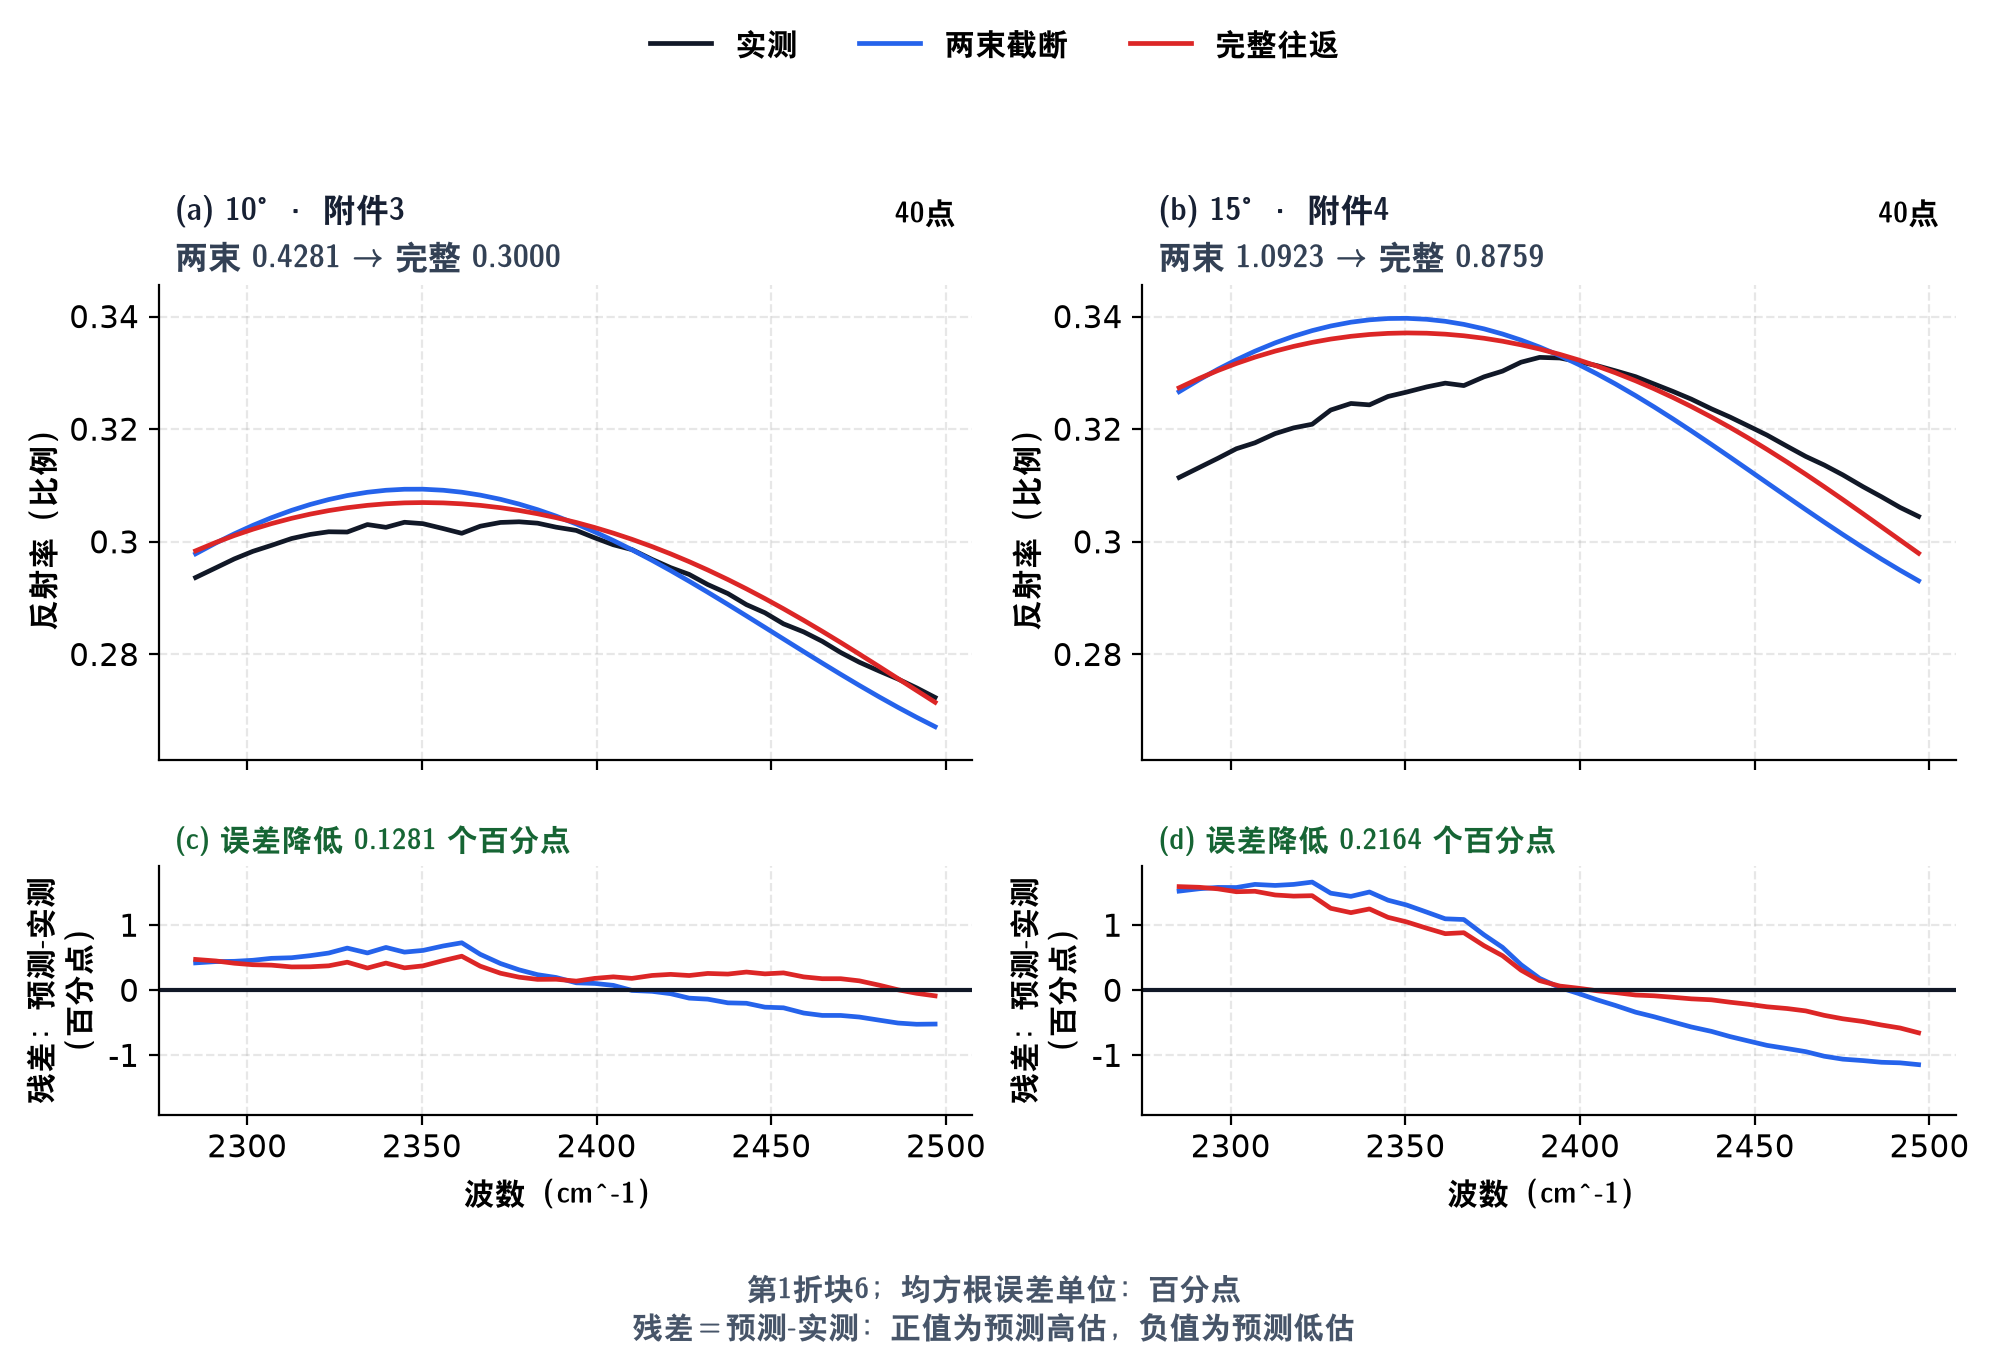
\includegraphics[width=0.8\textwidth]{../求解/问题3/图片/硅双角谱检验高阶贡献.png}
  \caption{硅两角高阶场预测残差存在差异}
  \label{fig:16}
\end{figure}
\endgroup

逐附件核对发现，硅附件三、四的高阶方案各在$2/4$个测试块上改善。早期对照曾因总体误差较低而保留完整往返，逐块检查却发现硅附件三仍有反向区段，因此保留各块的正负差值，表\ref{tab:supp-q3-blocks}与图\ref{fig:17}分别承担数值核对和方向比较。
% src:求解/问题3/结果/回炉轮3候选/仲裁闭环/20260910_131501_81623_建模公式/厚度结果.json:分材料验证.硅.逐角逐折逐块.0.完整相对两束下降_%;分材料验证.硅.逐角逐折逐块.1.完整相对两束下降_%;分材料验证.硅.逐角逐折逐块.2.完整相对两束下降_%;分材料验证.硅.逐角逐折逐块.3.完整相对两束下降_%;分材料验证.硅.逐角逐折逐块.4.完整相对两束下降_%;分材料验证.硅.逐角逐折逐块.5.完整相对两束下降_%;分材料验证.硅.逐角逐折逐块.6.完整相对两束下降_%;分材料验证.硅.逐角逐折逐块.7.完整相对两束下降_%
% src:交接/实验记录.json:852.类别;852.尝试;852.现象;852.决定

\begingroup
\setlength{\intextsep}{2pt}
\captionsetup{skip=3pt}
\begin{figure}[!htb]
  \centering
  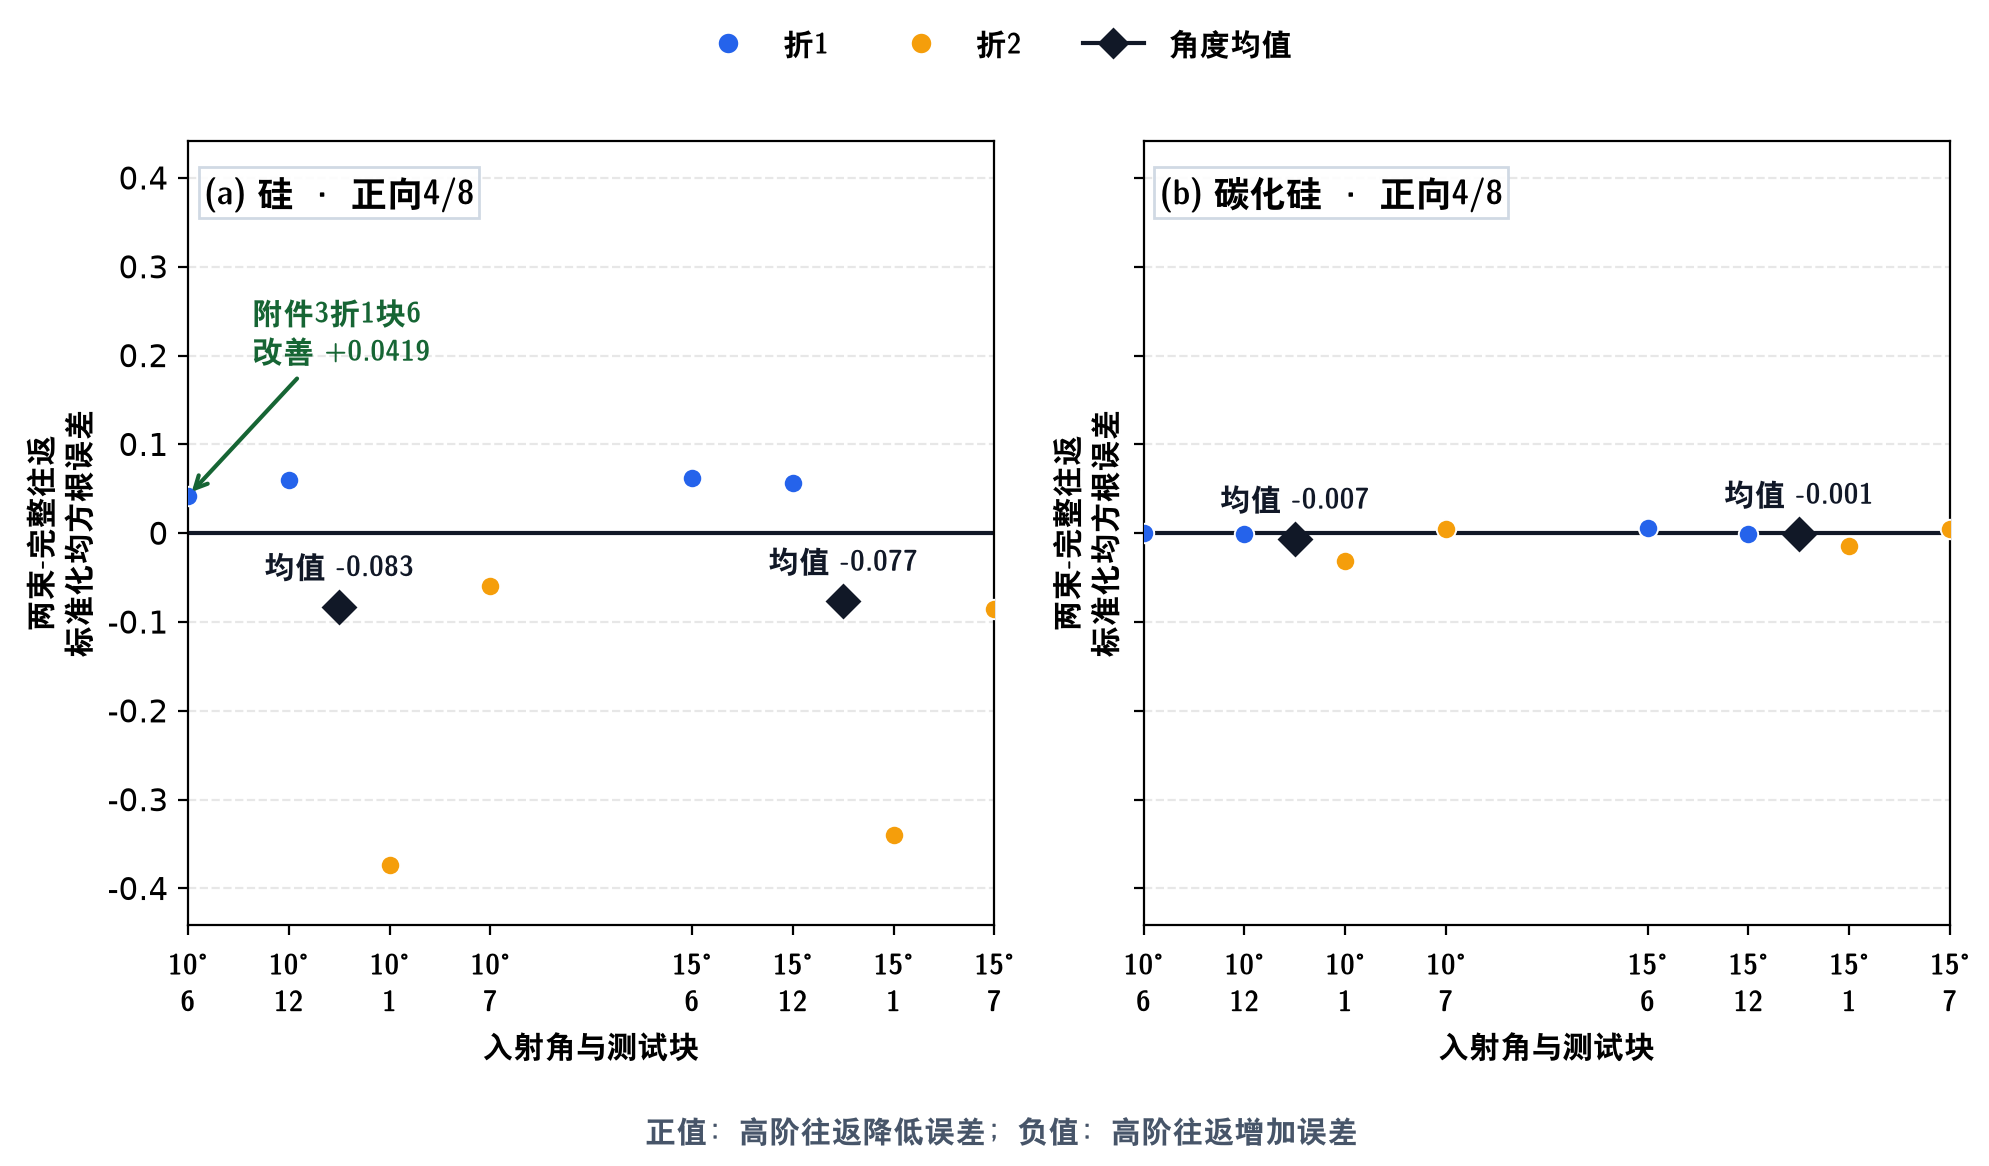
\includegraphics[width=0.8\textwidth]{../求解/问题3/图片/逐块对照区分两材料收益.png}
  \caption{两材料完整往返场的逐块误差改善}
  \label{fig:17}
\end{figure}
\endgroup

碳化硅附件一、二各有$2/4$个测试块出现高阶方案改善，正向收益均未贯穿全部区段。表\ref{tab:07}列出的物理可观测性与这些预测差异是两类证据。前者逐项检验式\eqref{eq:q3-cross-conditions}至式\eqref{eq:q3-resolution}的独立条件；后者比较留出光谱的预测误差。
% src:求解/问题3/结果/回炉轮3候选/仲裁闭环/20260910_131501_81623_建模公式/厚度结果.json:分材料验证.碳化硅.逐角逐折逐块.0.完整相对两束下降_%;分材料验证.碳化硅.逐角逐折逐块.1.完整相对两束下降_%;分材料验证.碳化硅.逐角逐折逐块.2.完整相对两束下降_%;分材料验证.碳化硅.逐角逐折逐块.3.完整相对两束下降_%;分材料验证.碳化硅.逐角逐折逐块.4.完整相对两束下降_%;分材料验证.碳化硅.逐角逐折逐块.5.完整相对两束下降_%;分材料验证.碳化硅.逐角逐折逐块.6.完整相对两束下降_%;分材料验证.碳化硅.逐角逐折逐块.7.完整相对两束下降_%

正向块并存负向块，说明高阶方案的预测收益没有贯穿四个附件。全量拟合中，硅与碳化硅的往返倍率模上界分别为$0.1441$和$0.0271$；表\ref{tab:q3-attachment-conditions}将这些模型内的非零返回与仍需测量的观测条件分列，不能从收敛直接跳到实验检出。
% src:求解/问题3/结果/公平对照.json:案例.0.场级数核验.最大往返乘子模;案例.3.场级数核验.最大往返乘子模

\begingroup
\footnotesize
\begin{longtable}{>{\centering\arraybackslash}p{0.06\textwidth}>{\centering\arraybackslash}p{0.12\textwidth}>{\centering\arraybackslash}p{0.19\textwidth}>{\centering\arraybackslash}p{0.20\textwidth}>{\centering\arraybackslash}p{0.27\textwidth}}
\caption{四附件的返回场与可观测条件}\label{tab:q3-attachment-conditions}\\
\hline
附件 & 正向块/总块 & 模型内可确认 & 谱形相容证据 & 未知观测条件\\
\hline
一 & $2/4$ & 非零返回、收敛 & 仅部分区段改善 & 相干、重叠、分辨及噪声\\
二 & $2/4$ & 非零返回、收敛 & 仅部分区段改善 & 相干、重叠、分辨及噪声\\
三 & $2/4$ & 非零返回、收敛 & 仅部分区段改善 & 相干、重叠、分辨及噪声\\
四 & $2/4$ & 非零返回、收敛 & 仅部分区段改善 & 相干、重叠、分辨及噪声\\
\hline
\end{longtable}
\endgroup
% src:求解/问题3/结果/回炉轮3候选/仲裁闭环/20260910_131501_81623_建模公式/厚度结果.json:分材料验证.硅.逐角逐折逐块.0.完整相对两束下降_%;分材料验证.硅.逐角逐折逐块.1.完整相对两束下降_%;分材料验证.硅.逐角逐折逐块.2.完整相对两束下降_%;分材料验证.硅.逐角逐折逐块.3.完整相对两束下降_%;分材料验证.硅.逐角逐折逐块.4.完整相对两束下降_%;分材料验证.硅.逐角逐折逐块.5.完整相对两束下降_%;分材料验证.硅.逐角逐折逐块.6.完整相对两束下降_%;分材料验证.硅.逐角逐折逐块.7.完整相对两束下降_%;分材料验证.碳化硅.逐角逐折逐块.0.完整相对两束下降_%;分材料验证.碳化硅.逐角逐折逐块.1.完整相对两束下降_%;分材料验证.碳化硅.逐角逐折逐块.2.完整相对两束下降_%;分材料验证.碳化硅.逐角逐折逐块.3.完整相对两束下降_%;分材料验证.碳化硅.逐角逐折逐块.4.完整相对两束下降_%;分材料验证.碳化硅.逐角逐折逐块.5.完整相对两束下降_%;分材料验证.碳化硅.逐角逐折逐块.6.完整相对两束下降_%;分材料验证.碳化硅.逐角逐折逐块.7.完整相对两束下降_%
% src:求解/问题3/结果/条件判定.json:必要条件

表中的非零返回与收敛均在所设光学模型内成立，相位关联、光束重叠和仪器响应则没有独立测量。图\ref{fig:roundtrip}中的返回路径对应$Bu$，相干叠加对应$\gamma_{mn}\eta_{mn}$；场幅逐次衰减本身不能确定卷积后的高阶交叉项是否高于噪声。

厚度影响也须单独识别。碳化硅同段厚度从$2.79$变为$2.83\ \mu\mathrm{m}$，折射率与损耗也同时改变，差值混合了参数补偿和往返影响。因此表\ref{tab:08}将模型对照与实际采用值分行。
% src:求解/问题3/结果/回炉轮3候选/仲裁闭环/20260910_131501_81623_建模公式/厚度结果.json:案例.6.最优.厚度_um;案例.7.最优.厚度_um;案例.6.最优.参数向量.1;案例.7.最优.参数向量.1;案例.6.最优.参数向量.4;案例.7.最优.参数向量.4

历史参数扰动中，碳化硅厚度变化介于$-1.6720$与$2.1261\ \mu\mathrm{m}$；图\ref{fig:19}保留这组重估对照，区别于固定参数的高阶场差，也未替换第二问的采用厚度。
% src:求解/问题3/结果/灵敏度.json:灵敏度_参数扰动.29.厚度变化_um;灵敏度_参数扰动.27.厚度变化_um;灵敏度_参数扰动.73.厚度变化_um;灵敏度_参数扰动.72.厚度变化_um

\begingroup
\setlength{\intextsep}{2pt}
\captionsetup{skip=3pt}

\endgroup

两项修正要求未同时成立，碳化硅维持$10.80\ \mu\mathrm{m}$及$0.64$--$18.11\ \mu\mathrm{m}$。图\ref{fig:20}并列两材料答案，硅的两折跨度与完整情景包络分开，碳化硅线段表示厚度重估范围。
% src:求解/问题3/结果/回炉轮3候选/仲裁闭环/20260910_131501_81623_建模公式/厚度结果.json:核心指标.碳化硅正式基准厚度_um;核心指标.碳化硅正式条件范围下限_um;核心指标.碳化硅正式条件范围上限_um
% src:求解/问题3/结果/条件判定.json:碳化硅条件分支.触发

\begingroup
\setlength{\intextsep}{2pt}
\captionsetup{skip=3pt}
\begin{figure}[!htb]
  \centering
  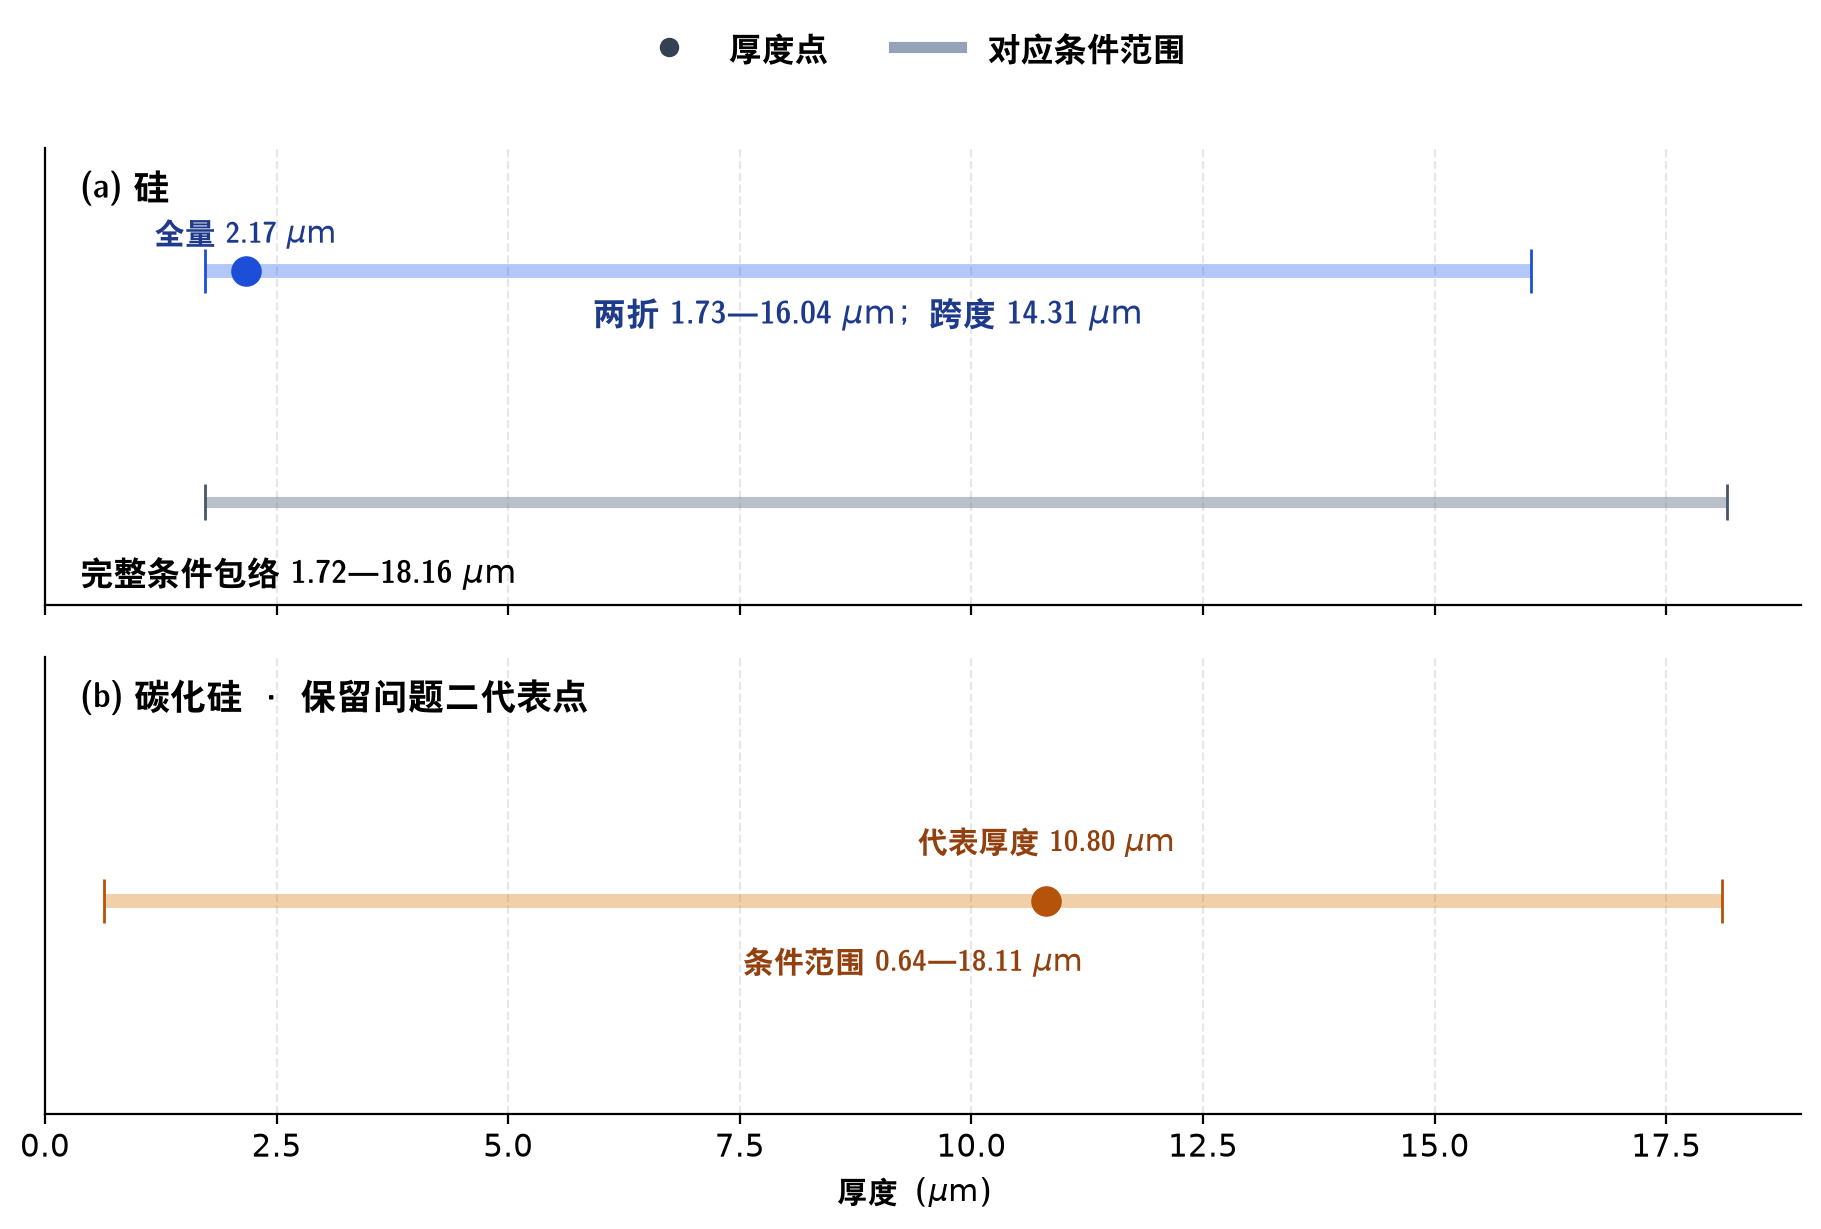
\includegraphics[width=0.8\textwidth]{../求解/问题3/图片/两材料厚度汇总保留条件.png}
  \caption{两材料厚度随切分与参数设置变化}
  \label{fig:20}
\end{figure}
\endgroup

硅采用完整往返场的全量拟合厚度，已计算的条件包络为$1.72$--$18.16\ \mu\mathrm{m}$，碳化硅沿用前问基准。包络由两模型全量、两折、近优候选及已算扰动的最外端点构成，是非概率的情景范围。
% src:求解/问题3/结果/回炉轮3候选/仲裁闭环/20260910_131501_81623_建模公式/厚度结果.json:核心指标.硅全量完整往返厚度_um;核心指标.硅折1完整往返条件厚度_um;核心指标.硅折2完整往返条件厚度_um;核心指标.硅已计算条件包络下限_um;核心指标.硅已计算条件包络上限_um;核心指标.碳化硅正式基准厚度_um;核心指标.碳化硅正式条件范围下限_um;核心指标.碳化硅正式条件范围上限_um

本问置信等级为低：硅次折相对训练均值劣化$11.30\%$，相对两束劣化$9.52\%$，两材料高阶收益跨折反向；同起点且均收敛的衬底扰动使厚度下降$13.83\%$，其他扰动的竞争分支差值跨零。已有结果给出有限光学条件下的最佳估计及描述性包络；已用于模型开发的测试区段承担探索性核对，独立同条件复算仍待补全，故尚不能确定唯一真厚度或概率区间。
% src:求解/问题3/结果/解读核验_回炉3_仲裁后.json:自检指标.硅折2相对训练均值改善_百分比;自检指标.硅折2相对两束改善_百分比;灵敏度.示例相对控制变化_百分比
% src:交接/结果声明_问题3.json:置信.等级;置信.理由

完整场的反射率测试经验覆盖率为$73.91\%$，低于名义$90\%$。下一章将反射率预测误差与厚度误差分开检验。
% src:求解/问题3/结果/回炉轮3候选/仲裁闭环/20260910_131501_81623_建模公式/厚度结果.json:预测区间.4.经验覆盖率;预测区间.4.平均区间宽度_比例;预测区间.5.经验覆盖率;预测区间.5.平均区间宽度_比例;预测区间.6.经验覆盖率;预测区间.6.平均区间宽度_比例;预测区间.7.经验覆盖率;预测区间.7.平均区间宽度_比例;预测区间.20.经验覆盖率;预测区间.20.平均区间宽度_比例;预测区间.21.经验覆盖率;预测区间.21.平均区间宽度_比例;预测区间.22.经验覆盖率;预测区间.22.平均区间宽度_比例;预测区间.23.经验覆盖率;预测区间.23.平均区间宽度_比例;预测区间.36.经验覆盖率;预测区间.36.平均区间宽度_比例;预测区间.37.经验覆盖率;预测区间.37.平均区间宽度_比例;预测区间.38.经验覆盖率;预测区间.38.平均区间宽度_比例;预测区间.39.经验覆盖率;预测区间.39.平均区间宽度_比例;预测区间.52.经验覆盖率;预测区间.52.平均区间宽度_比例;预测区间.53.经验覆盖率;预测区间.53.平均区间宽度_比例;预测区间.54.经验覆盖率;预测区间.54.平均区间宽度_比例;预测区间.55.经验覆盖率;预测区间.55.平均区间宽度_比例;预测区间.4.名义覆盖率
% src:求解/问题3/结果/回炉轮3候选/仲裁闭环/20260910_131501_81623_建模公式/厚度结果.json:逐块评分.4.测试点数;逐块评分.5.测试点数;逐块评分.6.测试点数;逐块评分.7.测试点数;逐块评分.20.测试点数;逐块评分.21.测试点数;逐块评分.22.测试点数;逐块评分.23.测试点数;逐块评分.36.测试点数;逐块评分.37.测试点数;逐块评分.38.测试点数;逐块评分.39.测试点数;逐块评分.52.测试点数;逐块评分.53.测试点数;逐块评分.54.测试点数;逐块评分.55.测试点数
% src:交接/结果声明_问题3.json:置信.等级;置信.理由

\par\endgroup
